\chapter{A plugin továbbfejlesztése}

\section{Kompozíció modellezése}
Állapottérképekkel rendszerek állapot és esemény alapú működését szoktuk leírni, legtöbbször azonban ezeket nem önmagukban hanem más modellek részeiként szoktuk használni, alacsonyabb szintű komponensek leírására, majd ezeket használva magasabb szintű komponenseket hozunk létre. A komponensek közti adatáramlások szintén fontos aspektusai egy rendszernek.


A Gamma keretrendszer egyik legkiemelkedőbb funkciója, hogy nem egyszerűen állapottérképek modellezésére ad lehetőséget, hanem ezek dekomponálására is. Az elemi komponens az állapotgép, ezeket felhasználva és a közöttük történő kommunikációk modellezésének segítségével összetett rendszereket vagyunk képesek leírni.

SysML-ben a rendszer funkcionális dekompozícióját Block Diagrammok segítségével végezzük, a komponensek kapcsolatát pedig Internal Block Diagrammokon tudjuk leírni.

\subsection{Szinktaktikai és szemantikai különbségek}

A két nyelv nagyon hasonlóan közelíti meg a rendszer dekomponálását. SysMLben blockokat azaz funkcionális egységeket definiáljuk és ezeket tartalmazási hierarchiába rendezzük magasabb szintű blokkokat definiálva, vagy ha top-bottom megközelítésben dolgozunk egy magasabb szintű blokkot bontunk fel részekre és a részeket még tovább kifejtük amennyire szükséges.

\begin{figure}[!ht]
	\centering
	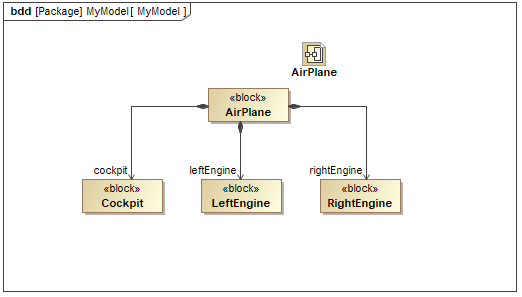
\includegraphics[width=75mm]{figures/examplebdd.png}
	\caption{Block Definition Diagram MagicDrawban}
\end{figure}

Ezt követően finomítjuk a modellt és a részek közötti kapcsolatokat is leírjuk. Ehhez portokat és konnektorokat használunk.
 
 \begin{figure}[!ht]
	\centering
	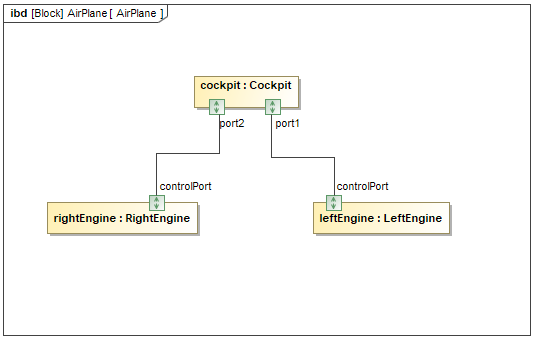
\includegraphics[width=75mm]{figures/exampleibd.png}
	\caption{Internal Block Diagram MagicDrawban}
\end{figure}

A Gammában a komponenseket és a kapcsolatokat köztük szöveges szintaxissal tudjuk leírni.

\begin{lstlisting}[language=bash,frame=single,float=!ht]
sync AirPlane [] {
	// Components of the composite model
	component leftEngine : LeftEngine
	component rightEngine : RightEngine

	// Connecting ports of components using channels
	channel [controller.PriorityControl] -o)- [prior.Control]
	channel [controller.SecondaryControl] -o)- [secondary.Control]

	channel [controller.PriorityPolice] -o)- [prior.PoliceInterrupt]
	channel [controller.SecondaryPolice] -o)- [secondary.PoliceInterrupt]
}
\end{lstlisting}


A Gamma megkülönbözteti a komponenseket aszerint, hogy ezek sorosan, vagy párhuzamosan működnek.
\subsection{Szinkron komponensek Gammában}
A Synchronous Component-ek olyan rendszereket reprezentálnak, melyek kommunikációja szinkron zajlik. A Gammában három féle elem van ami szinkron kommunikációt használ: StatechartDefinition, Synchronous Component, Cascade Synchronous Component. A komponensek szignálokkal kommunikálnak. Végrehajtás során a komponensek feldolgozzák a bejövő szignálokat és kimenő szignálokat állítanak elő, illetve megváltoztatják belső állapotukat.

\paragraph{Synchronous Composite Component:} a birtokolt komponensek végrehajtása ciklikusan történik, fixen meghatározott sorrendben, ami nem változik két végrehajtási ciklus között. A komponensek egy cikluson belül nem hatnak ki egymásra, az általuk küldött szignálok a következő ciklusban kerülnek feldolgozásra.

\paragraph{Cascade Composite Component:} ugyan azokat az elemeket tartalmazhatja, mint a Synchronous Composite Component, azonban komponensek által kibocsátott szignálok ugyan abban a végrehajtási ciklusban kerülnek feldolgozásra, fogadásra. Cascade komponensek esetében egy jólformáltsági kényszer, hogy komponensek közötti kommunikáció kör mentes legyen.

\subsection{Aszinkron komponensek Gammában}
Aszinkron komponensek olyan rendszereket reprezentálnak, ahol a komponensek egymástól független futnak. Az ilyen komponensek esetében a futási idő nem meghatározott. Aszinkron komponensek portokon keresztül kommunikálnak és pufferelt üzeneteket küldenek egymásnak. A Gammában kétféle aszinkron komponens van: Asynchronous Composite Component, Synchronous Component Wrappe

\paragraph{Asynchronous Composite Component:} Ugyan azokat az elemeket tartalmazzák, mint a Synchronous Composite Component, azonban aszinkron elemek nem tartalmazhatnak szinkron elemeket, így a szinkron működésű komponenseket be kell csomagolni egy Synchronous Component Wrapper-be.

\paragraph{Synchronous Component Wrapper:} Kompozit komponensek becsomagolására szolgál ezáltal aszinkron szemantikát adva neki. A Wrapper implicit rendelkezik a becsomagolt komponens portjaival, továbbá tartalmaz egy üzenet sort, ami tárolja a fogadott üzeneteket. Az üzenet sornak meghatározható a mérete, a fogadható üzenetek típusai és ezek az ezek közti prioritások.


\subsection{Gamma profil MagicDraw-hoz}

A Gamma szemantikájának MagicDraw-ban történő alkalmazását UML profiling segítségével érdemes megvalósítani. Ehhez sztereotípiákat kell definiálni amelyeket alkalmazni lehet SysML és UML modell elemeken, ezzel jelezve, hogy ezekre a Gamma által definiált szemantika az értelmezendő.

A Gamma MagicDraw profil SysML modellekhez készült. Mivel a SysML maga is egy sztereotípiákat definiáló profil a Gamma profil elemei a blokk sztereotípiából származnak le.

TODO: profil ismertetése

\section{Opaque kifejezések}

UML-ben és SysML-ben lehetőségünk van egyes elemek szöveges leírására is. A szöveges definíciókat tartalmazó eleket Opaque Expression-öknek nevezzük.

A MagicDraw nem írja elő,hogy milyen nyelvtant kell alkalmazni őrfeltételek vagy Opaque Expression formájában megadott akciókhoz, bár specifikálhatóvá tesz néhányat a felhasználónak (java, C, OCL).

Éppen ezért a kötetlenség miatt a MagicDrawToGamma a Gammában is használatos nyelvtant használta az őrfeltételek értelmezéséhez. Ez jelentősen megkönnyítette a modellek feldolgozását hiszen ezeket a kifejezéseket nem kellett Gamma kifejezésekké transzformálni.

Ahhoz, hogy a plugin szélesebb rétegek szémára is használható legyen érdemes lenne egy olyan nyelvet használni, amit gyakran alkalmaznak SysML modellek esetében.

\section{Object Contraint Language}

Az Object Constraint Language (OCL) egy deklaratív szabály leíró nyelv amit elsősorban jólformáltsági kényszerek leírására használnak, de állapottérképek őrfeltételeiként is alkalmazhatóak.

Ennek a nyelvnek a használatát az is ösztönzi, hogy ez része az UML szabványnak, így az UML alapú modelleken (pl. SysML-en is) szabvány szerint alkalmazható.

\subsection{OCL kifejezések alkalmazása}

OCL kifejezések alkalmazhatók:

\begin{itemize}
	\item Osztályok és típusok invariánsaként egy metamodellben
	\item Sztereotípiák típusainak invariánsaiként
	\item Viselkedések pre- és postkondícióihoz
	\item \textbf{Őrfeltételek leírására}
	\item jólformáltsági kényszerekhez
	\item modell lekérdezésekhez
\end{itemize}

\paragraph{Példa:} A Person osztály példányaiban az 'age' attribútum értéke nem lehet negatív.

\begin{lstlisting}[language=OCL,frame=single]
	context Person inv: self.age >=0
\end{lstlisting}

\paragraph{Példa:}  Meeting osztály do metódusa akkor hívható meg, ha 'canDo' értéke igaz
\begin{lstlisting}[language=OCL,frame=single]
context Meeting::do()
pre: self.canDo = true
\end{lstlisting}

Őrfeltételekként való alkalmazásnál a kontextus az állapotátmenet kell, hogy legyen. A self pointer pedig az állapottérképre, illetve ennek típusára mutat.

\subsection{Eclipse OCL}

OCL kifejezések EMF-re parsolásához az Eclipse-nek létezik egy implementációja ami képes bármilyen metamodellből parsert példányosítani és EMF alapú modellt generálnia kifejezésekből.


